\section{Penggunaan Selenium}
%\par Disini kami mencoba menjalankan otomasi \textit{web testing} menggunakan \textit{python} dan dengan menggunakan \textit{IDE Spyder}.
%Langkah-langkahnya yaitu :
%\begin{enumerate}
%\item buka \textit{spyder} dan tampilan awalnya seperti ini :
%	\begin{figure}[H]
    	\centering
    	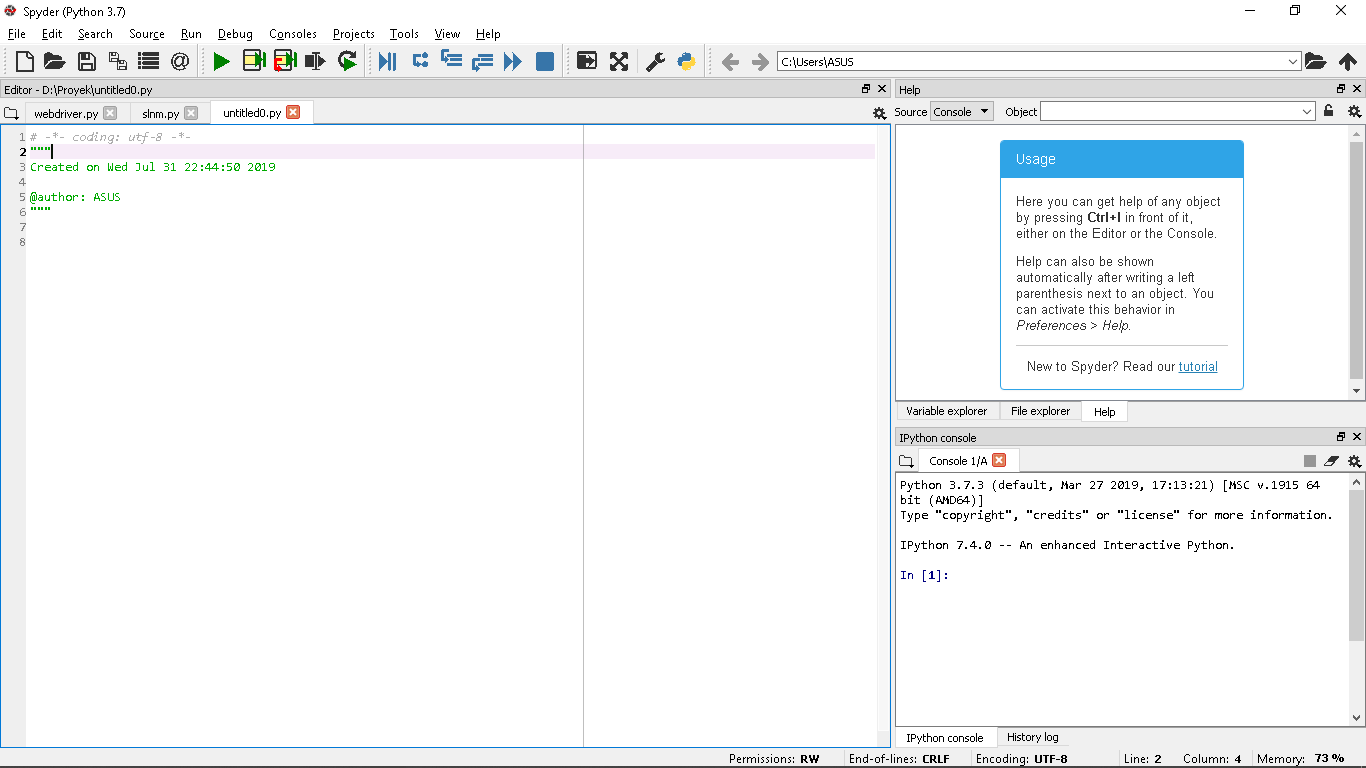
\includegraphics[scale=0.3]{figures/awalspy.png}
    	\caption{\textit{Tampilan awal spyder}}
    	\label{CLI}
	\end{figure}
	
\item kemudian ketikkan codingan :
\begin{lstlisting}[language=Python]
from selenium.webdriver import Firefox
from selenium.webdriver.firefox.options import Options
from selenium.webdriver.common.desired_capabilities import DesiredCapabilities
from selenium.webdriver.firefox.firefox_binary import FirefoxBinary

print("Masukkan Npm Anda:")
npm = input()
print("Masukkan Password SIAP Anda:")
paswd = input('')

opsi = Options()

opsi.headless = False
binary = FirefoxBinary("C:\\Program Files\\Mozilla Firefox\\firefox.exe")
cap = DesiredCapabilities().FIREFOX
cap['marionette'] = True

browser=Firefox(executable_path='geckodriver.exe',
options=opsi,capabilities=cap,firefox_binary=binary)
browser.get('http://siap.poltekpos.ac.id/siap/besan.depan.php')

name = browser.find_element_by_name('user_name')
word = browser.find_element_by_name('user_pass')
login = browser.find_element_by_name('login')


name.send_keys(npm)
word.send_keys(paswd)
login.click()

\end{lstlisting}

Penjelasan Codingan :
\begin{lstlisting}[language=Python]
from selenium.webdriver import Firefox
\end{lstlisting}
Yaitu Modul selenium webdriver mengimplementasikan kelas yang mendukung berbagai browser termasuk Firefox, Chrome, Internet Explorer, Safari, yang lain, dan RemoteWebDri	ver juga untuk menguji pada browser yang tersedia di mesin jarak jauh. Kita perlu mengimpor webdriver dari paket Selenium untuk menggunakan metode Selenium WebDriver.

\begin{lstlisting}[language=Python]
from selenium.webdriver.firefox.options import Options
\end{lstlisting}
Yaitu Opsi kelas dalam paket webdriver selenium firefox. opts adalah turunan dari kelas Opsi yang dipakai untuk program.

\begin{lstlisting}[language=Python]
from selenium.webdriver.common.desired_capabilities import DesiredCapabilities
\end{lstlisting}
Webdriver.common.desired_capabilities import DesiredCapabilities()
sebagai titik awal untuk membuat objek kemampuan yang diinginkan untuk meminta driver web jarak jauh untuk terhubung ke server selenium.

\begin{lstlisting}[language=Python]
from selenium.webdriver.firefox.firefox_binary import FirefoxBinary
\end{lstlisting}
Yaitu untuk mengimport FirefoxBinary atau lokasi dari si firefox.

\begin{lstlisting}[language=Python]
print("Masukkan Npm Anda:")
npm = input()
print("Masukkan Password SIAP Anda:")
paswd = input('')

\end{lstlisting}
ini merupakan inputan \textit{user}

\begin{lstlisting}[language=Python]
browser.get('http://siap.poltekpos.ac.id/siap/besan.depan.php')
\end{lstlisting}
Browser.get metode akan menavigasi ke halaman yang diberikan oleh URL. WebDriver akan menunggu hingga halaman dimuat penuh (yaitu, "onload" telah diaktifkan) sebelum mengembalikan kontrol ke tes atau skrip.

\item Setelah membuat Tambahan Codingan  seperti diatas untuk merunning program anda tekan run pada bar diatas.
\begin{figure}[H]
    	\centering
    	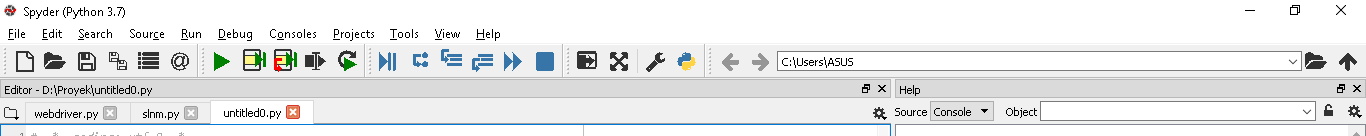
\includegraphics[scale=0.3]{figures/run1.png}
    	\caption{\textit{Running spyder}}
    	\label{CLI}
	\end{figure}

\newpage

\item Pada saat di run akan terlihat pada IPython console seperti gambar 
\begin{figure}[H]
    	\centering
    	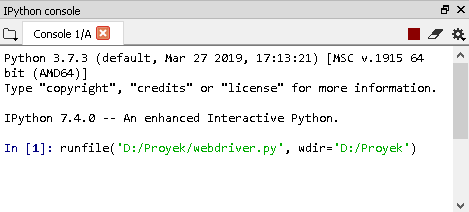
\includegraphics[scale=0.5]{figures/run2.png}
    	\caption{\textit{Running spyder console}}
    	\label{CLI}
	\end{figure}

\item Saat kotak yang ditandai pada gambar dibawah, berwarna merah artinya proses running program tersebut masih berjalan.
\begin{figure}[H]
    	\centering
    	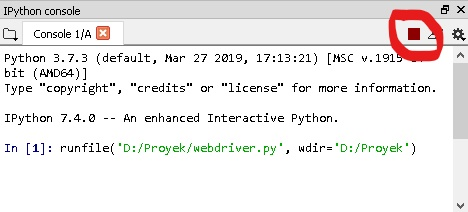
\includegraphics[scale=0.5]{figures/run3.png}
    	\caption{\textit{Running masih berjalan}}
    	\label{CLI}
	\end{figure}

\item Jika proses \textit{running} sudah selesai tampilannya akan seperti ini. Berarti Tambahan Codingan tersebut berhasil di \textit{running} dan tidak terdapat \textit{error}.
\begin{figure}[H]
    	\centering
    	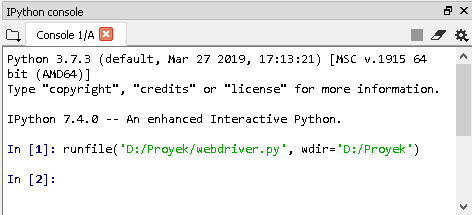
\includegraphics[scale=0.5]{figures/run4.png}
    	\caption{\textit{Running selesai}}
    	\label{CLI}
	\end{figure}

\item Setelah program di run akan otomatis membuka Mozila Firefox dan akan langsung membuka website siap.poltekpos.ac.id secara otomatis.
\begin{figure}[H]
    	\centering
    	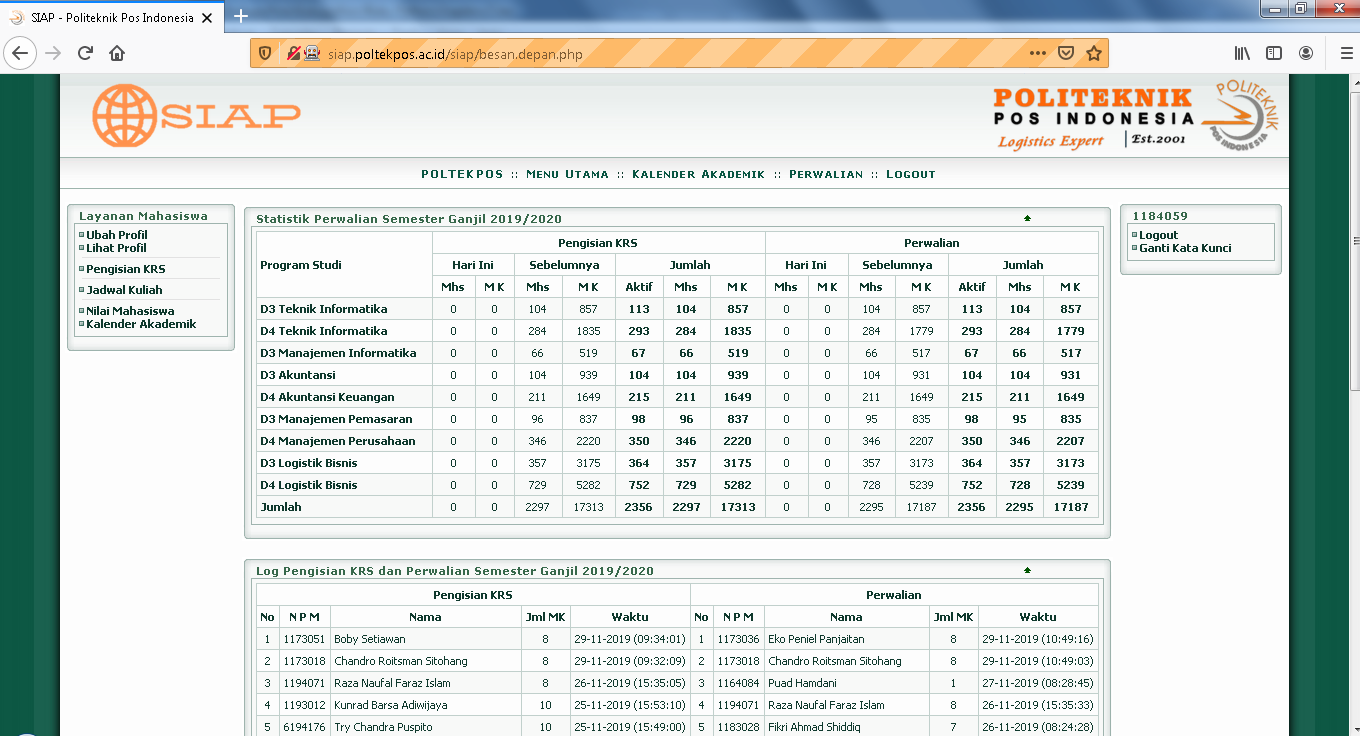
\includegraphics[scale=0.3]{figures/run5.png}
    	\caption{\textit{Tampilan siap.poltekpos}}
    	\label{CLI}
	\end{figure}


\end{enumerate}

\subsection{Cara find element atau class }
\par Selanjutnya kami akan mencoba \textit{Find Element} yang terdapat pada \textit{website} tersebut. Sebelumnya anda harus mengetahui apa saja jenis-jenis \textit{element} dan berikut adalah contoh dari \textit{element}.

\begin{enumerate}
\item find_element_by_id
\par Gunakan ini ketika Anda tahu atribut id suatu elemen. Dengan strategi ini, elemen pertama dengan nilai atribut id yang cocok dengan lokasi akan dikembalikan.
contoh :
\begin{lstlisting}[language=Python]
<form id="login">
   login = Browser.find_element_by_id('login')
\end{lstlisting}

\item find_element_by_name
\par Gunakan ini ketika Anda tahu atribut nama elemen. Dengan strategi ini, elemen pertama dengan nilai atribut nama yang cocok dengan lokasi akan dikembalikan.
contoh :
\begin{lstlisting}[language=Python]
<input name ="username" type="text" />
  username = Browser.find_element_by_name('username')
\end{lstlisting}

\item find_element_by_xpath
\par XPath adalah bahasa yang digunakan untuk menemukan node dalam dokumen XML. Karena HTML dapat menjadi implementasi XML (XHTML), pengguna Selenium dapat memanfaatkan bahasa yang kuat ini untuk menargetkan elemen dalam aplikasi web mereka. Dan cara mendapatkan xpath adalah inspect website tersebut dan klik kanan pada element yang ingin di cari dan klik copy dan disana ada copy Xpath.
contoh :
\begin{lstlisting}[language=Python]
" ('/html/body/table/tbody/tr[5]/td/table[3]/tbody/tr[1]/td[2]/p[1]/table/tbody/tr/td[3]/select').click()" 
 browser.find_element_by_xpath('/html/body/table/tbody/tr[5]/td/table[3]/tbody/tr[1]/td[2]/p[1]/table/tbody/tr/td[3]/select').click()
\end{lstlisting}

\item find_element_by_link_text
\par Gunakan ini ketika Anda tahu teks tautan yang digunakan dalam tag jangkar. Dengan strategi ini, elemen pertama dengan nilai teks tautan yang cocok dengan lokasi akan dikembalikan. 
contoh :
\begin{lstlisting}[language=Python]
<a href="continue.html">Continue</a>
Continue = Browser.find_element_by_link_text('Continue')
\end{lstlisting}

\item find_element_by_tag_name
\par Gunakan ini ketika Anda ingin mencari elemen dengan nama tag. Dengan strategi ini, elemen pertama dengan nama tag yang diberikan akan dikembalikan.
contoh :
\begin{lstlisting}[language=Python]
<strong>Hello</strong> 
Strong = Browser.find_element_by_tag_name('strong')
\end{lstlisting}

\item find_element_by_class_name
\par Gunakan ini ketika Anda ingin mencari elemen dengan nama atribut kelas. Dengan strategi ini, elemen pertama dengan nama atribut kelas yang cocok akan dikembalikan. 
contoh :
\begin{lstlisting}[language=Python]
<p class="body">Halo.</p>
body = Browser.find_element_by_class_name('body')
\end{lstlisting}

\item find_element_by_css_selector
\par Gunakan ini ketika Anda ingin mencari elemen dengan sintaks pemilih CSS. Dengan strategi ini, elemen pertama dengan pemilih CSS yang cocok akan dikembalikan. 
contoh : 
\begin{lstlisting}[language=Python]
<p class="body">Halo.</p> 
body = Browser.find_element_by_class_name('p.body')
\end{lstlisting}

\end{enumerate}

\subsection{Mengambil element dari web siap.poltekpos.ac.id}
\par Setelah mengenal tentang element mari kita mencoba mencari element pada website siap.poltekpos.ac.id

\newpage

\begin{enumerate}
\item Disini kami mencoba untuk mengisi data \textit{user} pada \textit{login}.
\begin{figure}[H]
    	\centering
    	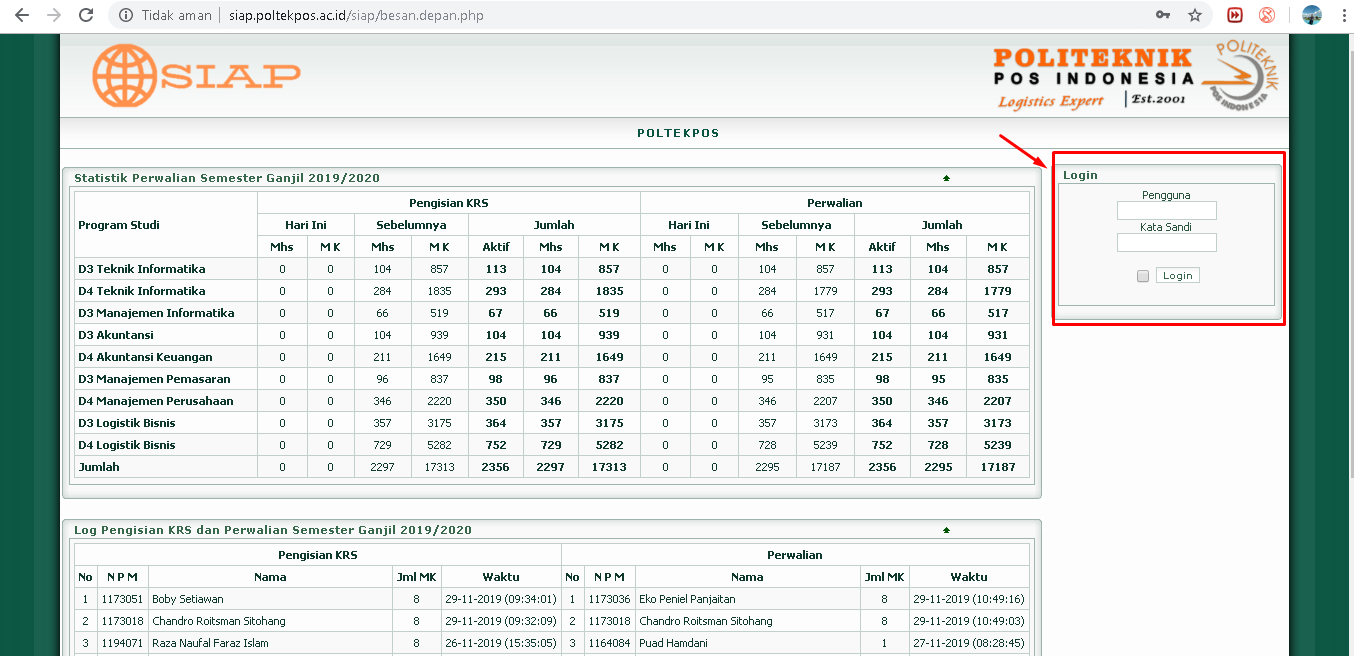
\includegraphics[scale=0.3]{figures/siap.png}
    	\caption{\textit{Tampilan siap.poltekpos}}
    	\label{CLI}
	\end{figure}
\item Untuk mencari elementnya arahkan cursor ke \textit{login} pengguna, kata sandi, dan login. lalu klik kanan dan \textit{inspect}, disini kami menggunakan element_by_name.

\begin{figure}[H]
    	\centering
    	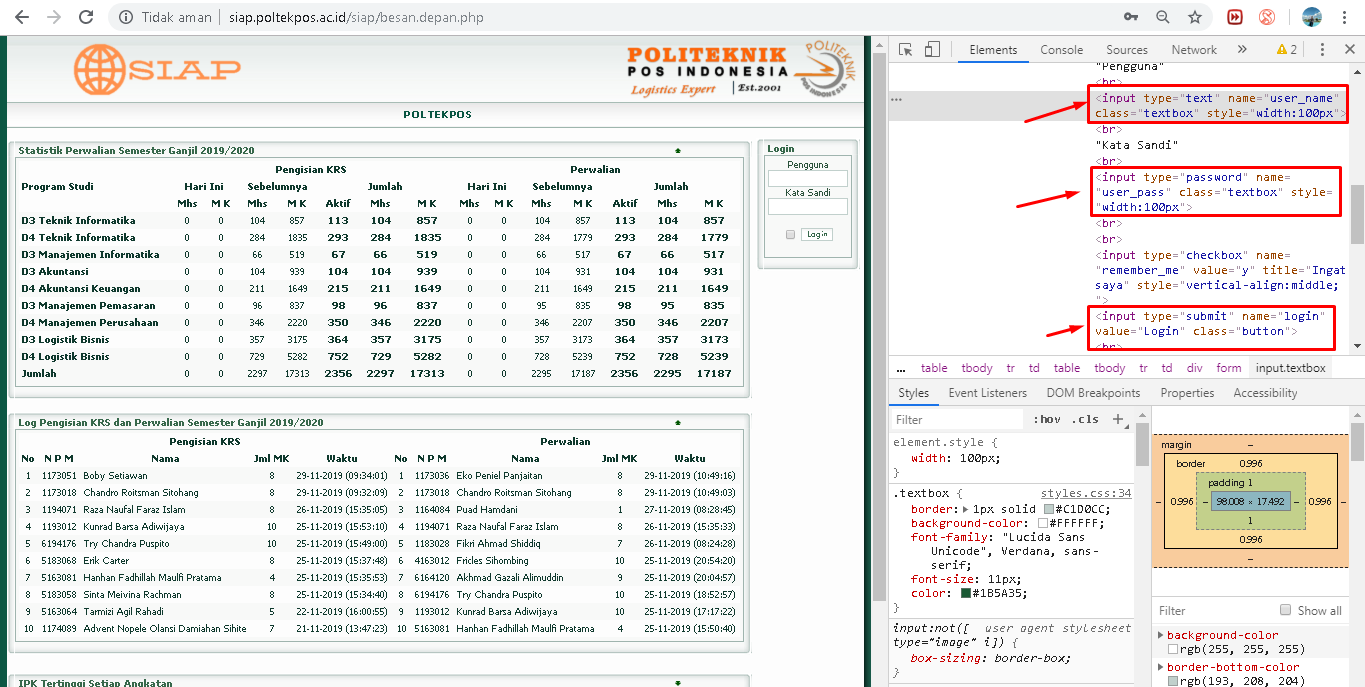
\includegraphics[scale=0.3]{figures/inspect1.png}
    	\caption{\textit{inspect element by name}}
    	\label{CLI}
	\end{figure}
	
Tambahan Codingan :
\begin{lstlisting}[language=Python]
name = browser.find_element_by_name('user_name')
word = browser.find_element_by_name('user_pass')
login = browser.find_element_by_name('login')

\end{lstlisting}

\newpage

Hasil :
\begin{figure}[H]
    	\centering
    	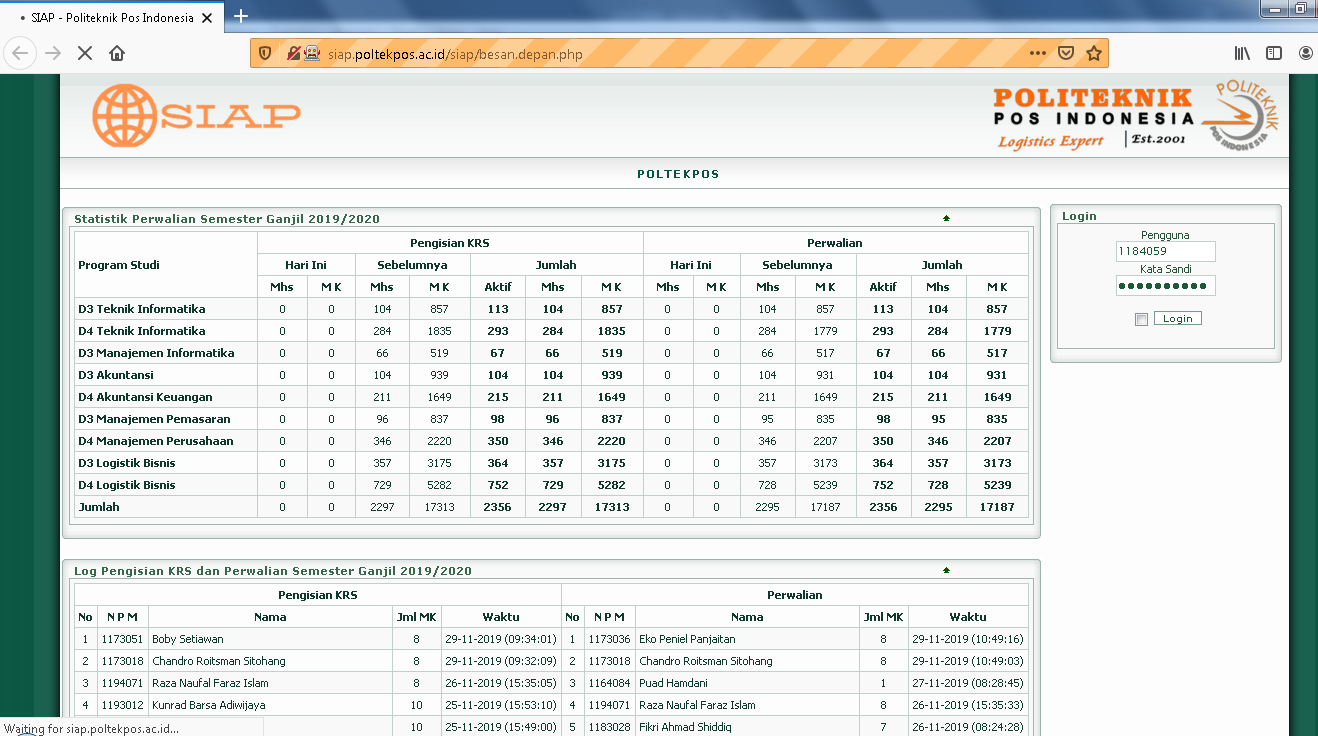
\includegraphics[scale=0.3]{figures/hasillogin.png}
    	\caption{\textit{Tampilan loading login}}
    	\label{CLI}
	\end{figure}
	
Hasil :
\begin{figure}[H]
    	\centering
    	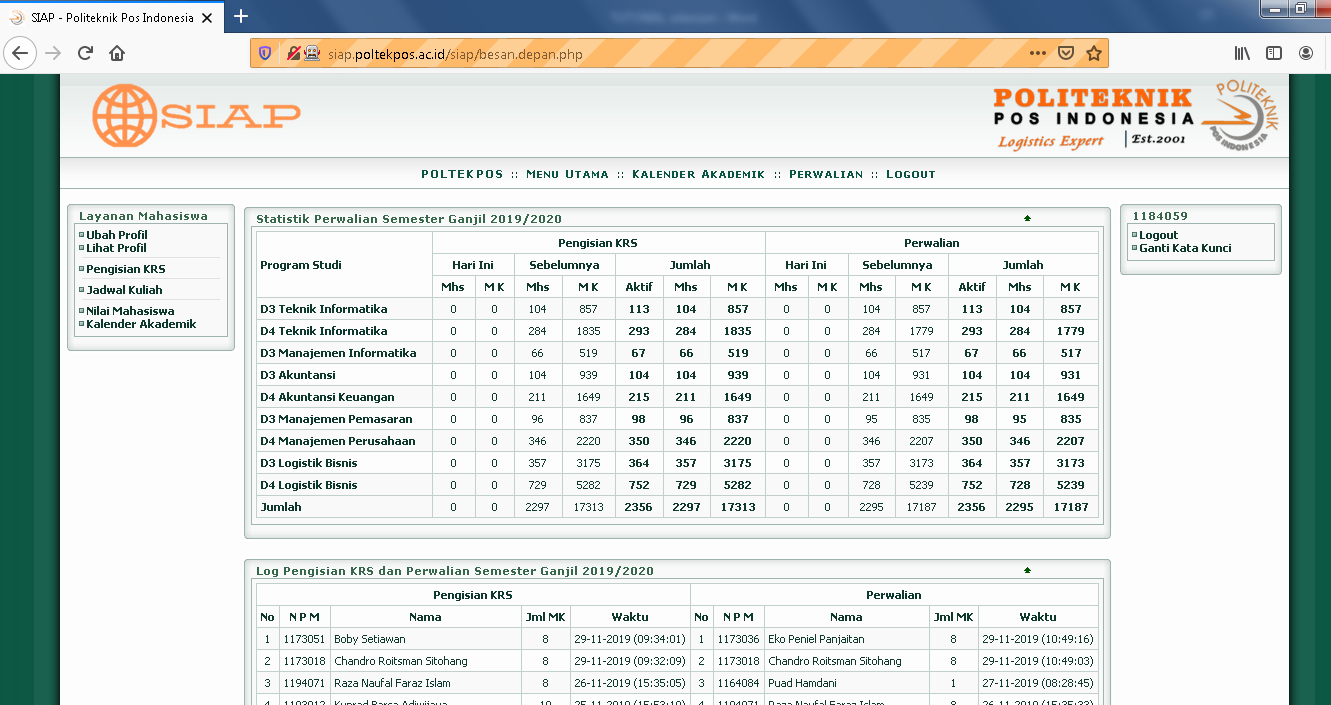
\includegraphics[scale=0.3]{figures/hasillogin1.png}
    	\caption{\textit{Tampilan login}}
    	\label{CLI}
	\end{figure}


\item Pada layanan mahasiswa, kami mencoba untuk melihat nilai mahasiswa secara otomatis. Dengan cara yaitu klik kanan pada nilai mahasiswa, kemudian pilih \textit{inspect}.
\begin{figure}[H]
    	\centering
    	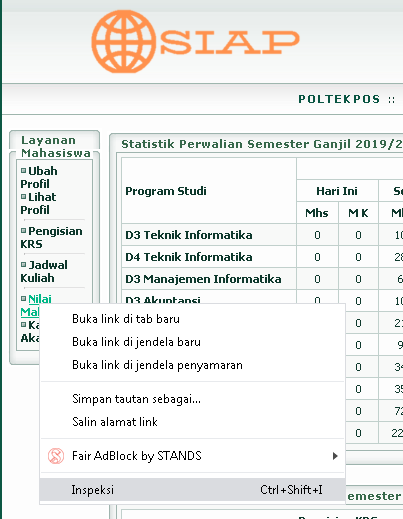
\includegraphics[scale=0.5]{figures/nilai1.png}
    	\caption{\textit{inspect element nilai mahasiswa}}
    	\label{CLI}
	\end{figure}

\newpage

Disini kami mengambil \textit{element by xpath}
\begin{figure}[H]
    	\centering
    	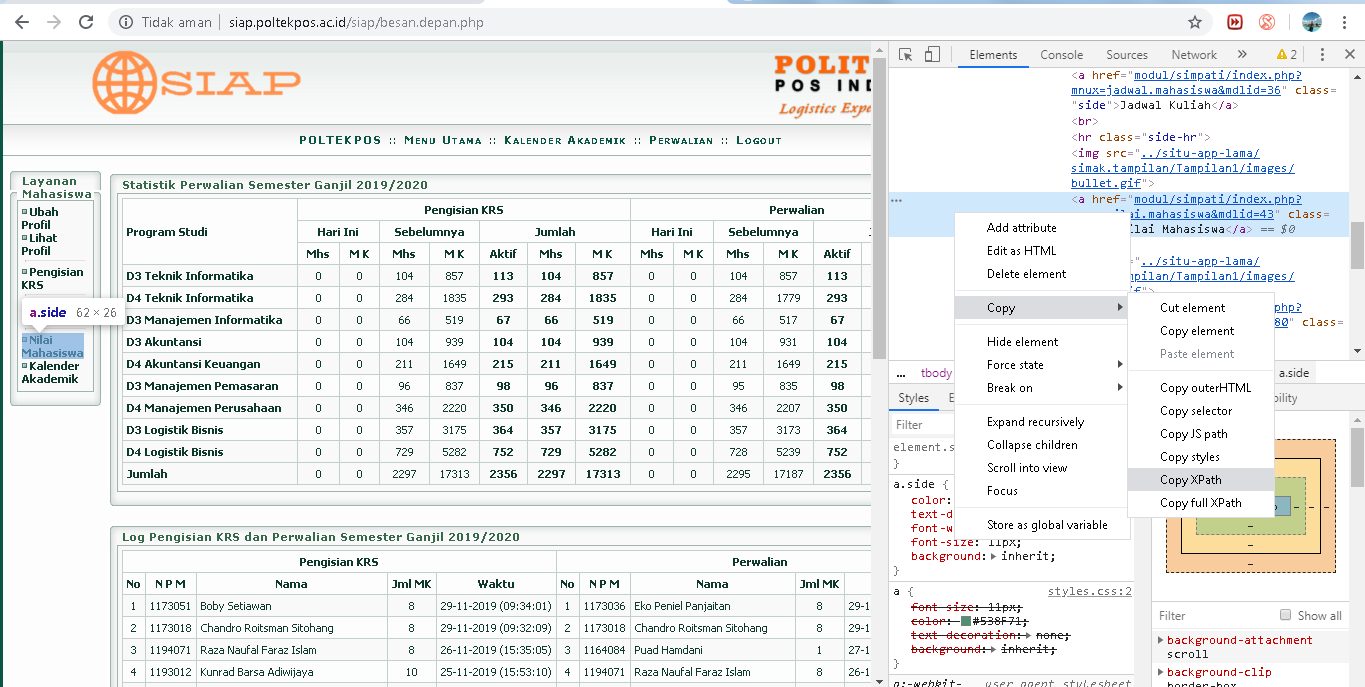
\includegraphics[scale=0.3]{figures/nilai2.png}
    	\caption{\textit{inspect element by xpath}}
    	\label{CLI}
	\end{figure}
	
Tambahan codingan :
\begin{lstlisting}[language=Python]
nilai= browser.find_element_by_xpath("/html/body/table/tbody/tr[5]/td/table[1]/tbody/tr/td[1]/table[2]/tbody/tr[1]/td[2]/a[5]").click()
\end{lstlisting}

Hasil :
\begin{figure}[H]
    	\centering
    	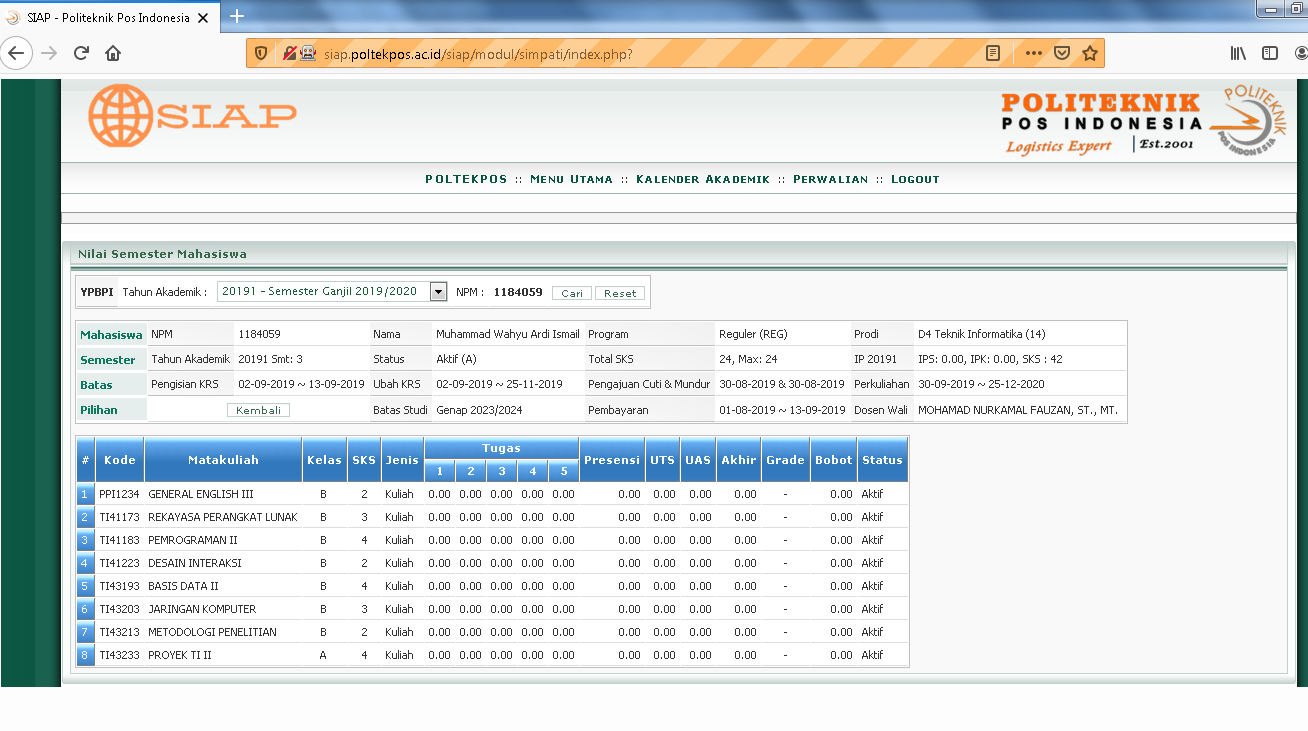
\includegraphics[scale=0.3]{figures/hasilnilai1.png}
    	\caption{\textit{Tampilan nilai semester mahasiswa}}
    	\label{CLI}
	\end{figure}

\newpage
	
\item Kemudian pada kolom tahun akademik, klik kanan dan pilih \textit{inspect}
\begin{figure}[H]
    	\centering
    	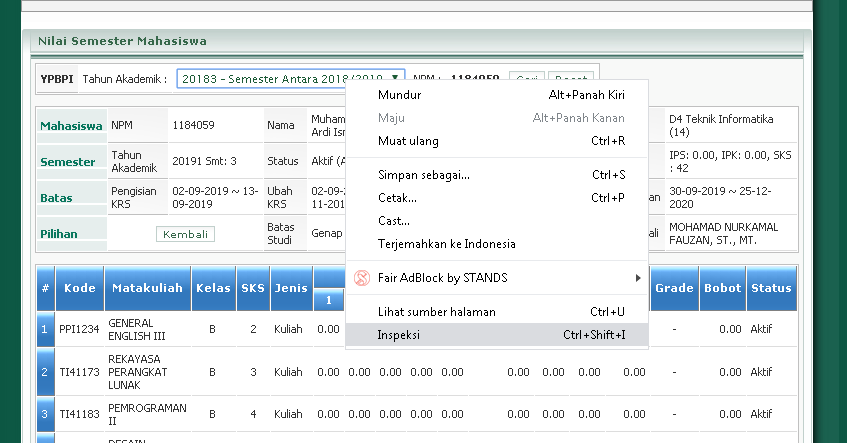
\includegraphics[scale=0.3]{figures/tahun1.png}
    	\caption{\textit{inspect element tahun akademik}}
    	\label{CLI}
	\end{figure}
	
Disini kami mengambil \textit{element by xpath} pada semester genap 2018/2019
\begin{figure}[H]
    	\centering
    	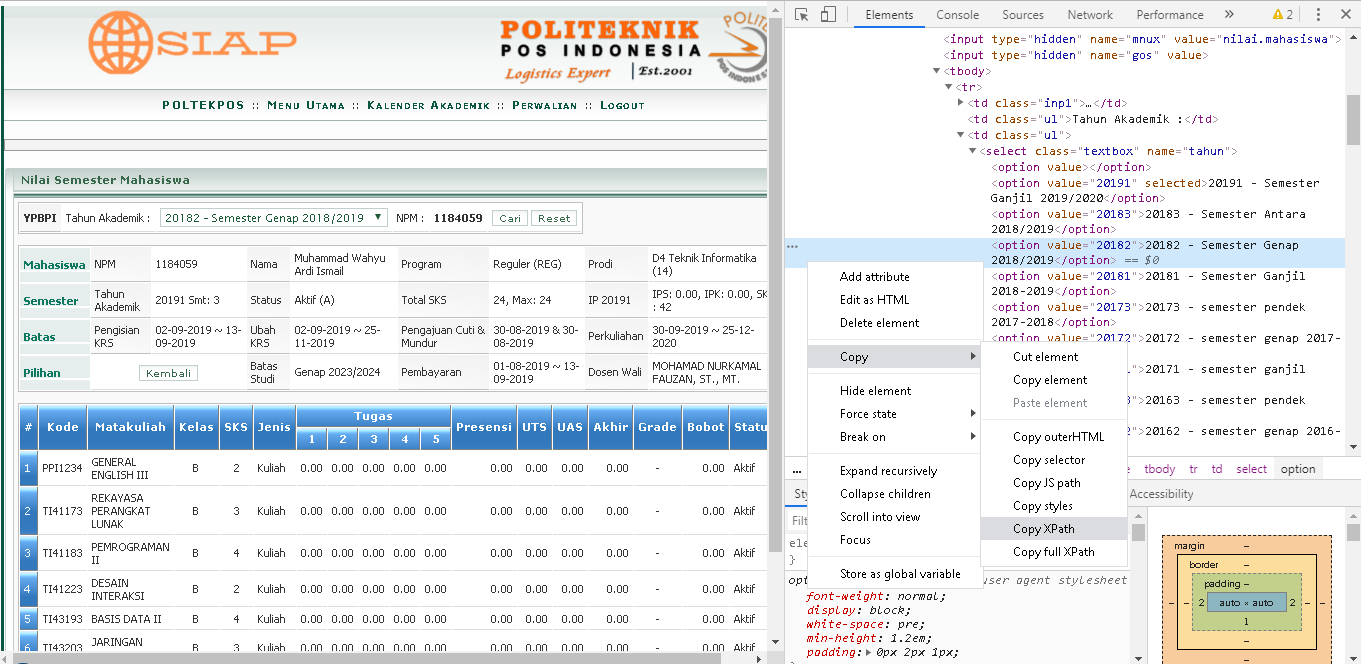
\includegraphics[scale=0.3]{figures/semestergenap.png}
    	\caption{\textit{inspect element by xpath semster genap}}
    	\label{CLI}
	\end{figure}

Tambahan codingan :
\begin{lstlisting}[language=Python]
nilai semester genap =browser.find_element_by_xpath('/html/body/table/tbody/tr[5]/td/table[3]/tbody/tr[1]/td[2]/p[1]/table/tbody/tr/td[3]/select/option[4]').click()
\end{lstlisting}

\newpage

Hasil :
\begin{figure}[H]
    	\centering
    	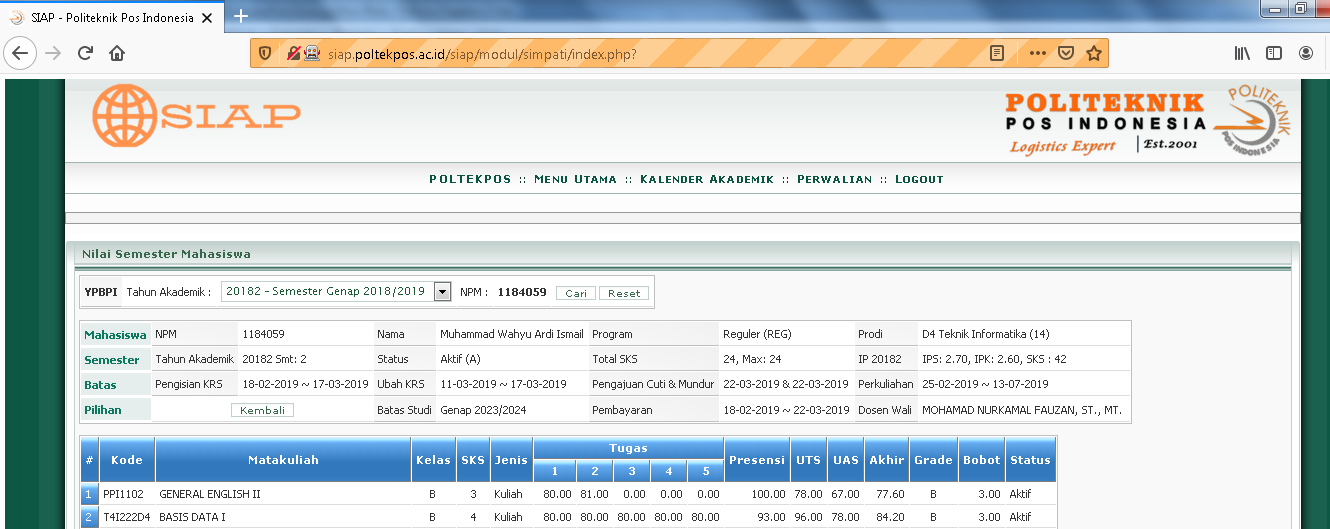
\includegraphics[scale=0.3]{figures/hasilnilai2.png}
    	\caption{\textit{Tampilan nilai semester genap 2018/2019}}
    	\label{CLI}
	\end{figure}



\item kemudian klik find cari dengan cara klik kanan pilih \textit{inspect}
\begin{figure}[H]
    	\centering
    	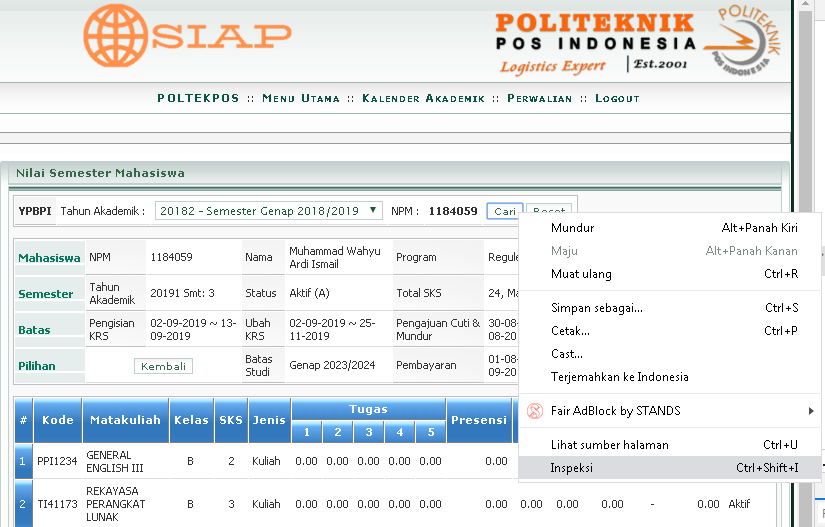
\includegraphics[scale=0.3]{figures/cari1.png}
    	\caption{\textit{inspect element cari}}
    	\label{CLI}
	\end{figure}
	
Disini kami mengambil \textit{element by class name}, \textit{class name} yaitu \textit{button}.
\begin{figure}[H]
    	\centering
    	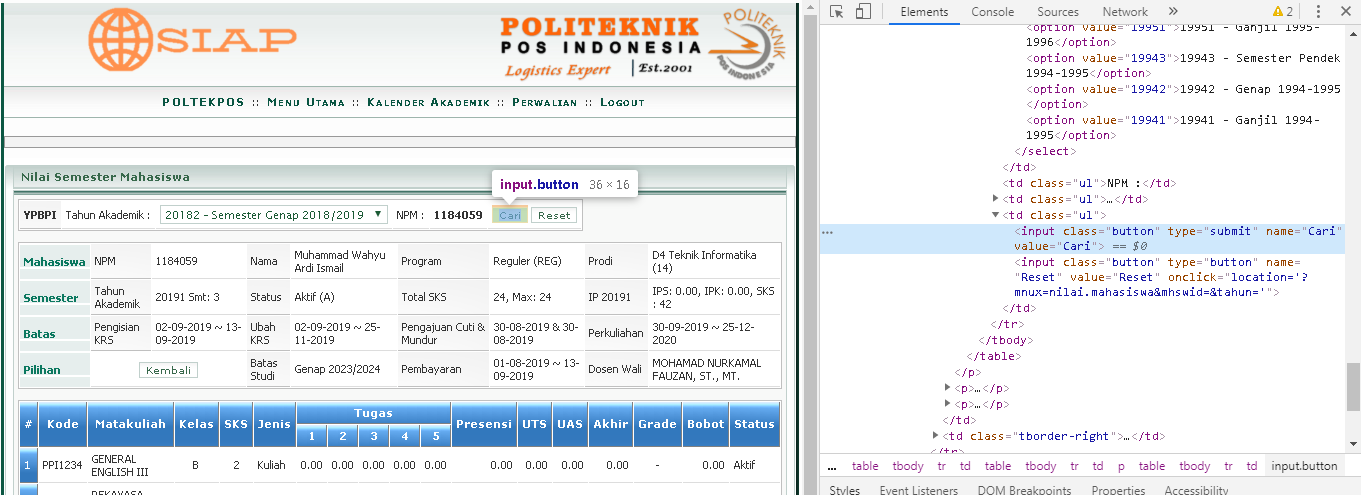
\includegraphics[scale=0.3]{figures/button1.png}
    	\caption{\textit{inspect element by class name cari}}
    	\label{CLI}
	\end{figure}

Tambahan codingan :
\begin{lstlisting}[language=Python]
cari = browser.find_element_by_class_name('button').click()
\end{lstlisting}


\item codingan keseluruhan :
\begin{lstlisting}[language=Python]
from selenium.webdriver import Firefox
from selenium.webdriver.firefox.options import Options
from selenium.webdriver.common.desired_capabilities import DesiredCapabilities
from selenium.webdriver.firefox.firefox_binary import FirefoxBinary

print("Masukkan Npm Anda:")
npm = input()
print("Masukkan Password SIAP Anda:")
paswd = input('')

opsi = Options()

opsi.headless = False
binary = FirefoxBinary("C:\\Program Files\\Mozilla Firefox\\firefox.exe")
cap = DesiredCapabilities().FIREFOX
cap['marionette'] = True

browser=Firefox(executable_path='geckodriver.exe',
options=opsi,capabilities=cap,firefox_binary=binary)
browser.get('http://siap.poltekpos.ac.id/siap/besan.depan.php')

name = browser.find_element_by_name('user_name')
word = browser.find_element_by_name('user_pass')
login = browser.find_element_by_name('login')


name.send_keys(npm)
word.send_keys(paswd)
login.click()

nilai = browser.find_element_by_xpath("/html/body/table/tbody/tr[5]/td/table[1]/tbody/tr/td[1]/table[2]/tbody/tr[1]/td[2]/a[5]").click()
semester1 = browser.find_element_by_xpath('/html/body/table/tbody/tr[5]/td/table[3]/tbody/tr[1]/td[2]/p[1]/table/tbody/tr/td[3]/select/option[4]').click()
cari = browser.find_element_by_class_name('button').click()

\end{lstlisting}


\end{enumerate}


 












